This section will provide an overview on computer vision, object detection and tracking on digital images, neural networks, Kalman filter, and modeling and control of a gimbal system.

\section{Digital Images}
To begin an explanation on computer vision, we need to understand how digital images are made. \citen{Gonzalez3} shows that digital images are obtained through sensors arranged in the form of a 2-D (two dimensional) array, and the response of each sensor is proportional to the integral of the light energy projected onto the surface of the sensor. When the sensors captures the image, two processes are made to digitize, Sampling is used to digitize the coordinates and Quantization for intensity (amplitude). The resulting representation of digital images in grayscale can be approximated by a traditional matrix, where each element represents a pixel. Color images can be represented as a tensor of order three. ``A tensor is a multidimensional array... a first-order tensor is a vector, a second-order tensor is a matrix, and tensors of order three or higher are called higher-order tensors'' \cite{Tensor}. Figure \ref{ImageTensor} illustrates color images as a tensor in the RGB (Red, Blue, Green) system.

\begin{figure}[h]
	\centering
	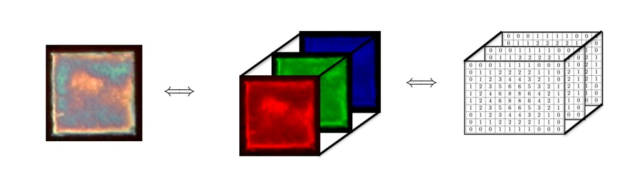
\includegraphics{Cap2/ImagemCor.eps}
	\caption{Color Image represented as a tensor. Source: \citen{ColorImage}.}\label{ImageTensor}
\end{figure}

It is important to have this consideration when thinking about the input datasets.

\section{Machine Learning}
\citen{Murphy-2012} defines machine learning as a set of methods that can automatically detect patterns in data, and then use the uncovered patterns to predict future data, or to perform other kinds of decision making under uncertainty (such as planning how to collect more data). In this field, Learning Algorithms can be defined as proposed by \citen{Mitchell}: ``A computer program is said to learn from experience $E$ with respect to some class of tasks $T$ and performance measure $P$, if its performance at tasks in $T$, as measured by $P$, improves with experience $E$''. Machine learning can be divided as Supervised machine mearning and Unsupervised machine mearning. In the Supervised learning the algorithm is presented with labeled datasets, explicitly defining the desired input-output behavior of the model. On the other hand, in Unsupervised learning no labels are given, so the patterns must be found in data in order to determine how to cluster the information and generate/create labels for predicting and classifying new data. For more information, refer to \citen{Brunton_Kutz_2022}.

\section{Neural Networks}
\label{Neural Networks}
As stated in \citen{Brunton_Kutz_2022}, the Nobel Prize winning work of \citen{hubel1962receptive} on the primary visual cortex of cats served as inspiration for NNs (neural networks). NNs specifically optimize over the compositional function
\begin{equation}
	\underset{\mathbf{A}_{j}}{\textrm{argmin}}(f_{M}(\mathbf{A}_{M},...,f_{2}(\mathbf{A}_{2},f_{1}(\mathbf{A}_{1},\mathbf{x}))...)+\lambda g(\mathbf{A}_{j})),
\end{equation}
where each matrix $\mathbf{A}_{k}$ refers to the weights connecting the NN from the $k$-th to the $(k+1)$-th layer. Being a massively under-determined system, $\lambda g(\mathbf{A}_{j})$ (called penalization) tries to regulate it. Some of the algorithms used to solve this equation are backpropagation (section \ref{Backpropagation Algorithm}) and stochastic gradient descent (section \ref{SecaoStocastica}).  The number of layers, dimension, connections and other design features of NNs are being studied and may vary according the application. Figure \ref{NN_generic} shows the architecture of a generic NN mapping $\mathbf{x}$ to $\mathbf{y}$.

\begin{figure}[h]
	\centering
	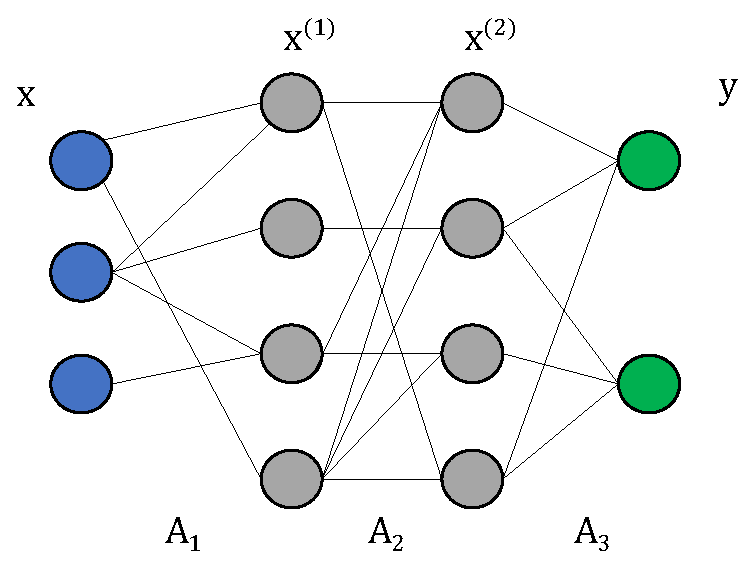
\includegraphics[scale = 0.6]{Cap2/NN.eps}
	\caption{An example of NN architecture. Source: \citen{Brunton_Kutz_2022}.}\label{NN_generic}
\end{figure}

If we consider a linear mapping between each layer, it becomes a linear system that can be represented as $\mathbf{A}_{k}\mathbf{x}^{(k-1)} = \mathbf{x}^{(k)}$. When working with nonlinear transformation from input to output, the mapping in each layer can be represented as
\begin{equation}
	\mathbf{x}^{(k)} = f(\mathbf{A}_{k},\mathbf{x}^{(k-1)}),	
\end{equation}
where $f$ is called an activation function, and works as a transfer function. Linear, sigmoid, tanh, and rectified linear unit (ReLU) are some of the commonly used activation functions, respectively expressed as
\begin{equation}
	\label{linear}
	f(x) = x,
\end{equation}
\begin{equation}
	\label{sigmoid}
	f(x) = \frac{1}{1+\exp(-x)},
\end{equation}
\begin{equation}
	\label{tanh}
	f(x) = \tanh(x),
\end{equation}
\begin{equation}
	\label{ReLU}
	f(x) = 
	\begin{cases}
		0, &   x \leq 0, \\
		x, &   x > 0.
	\end{cases}
\end{equation}

\section{Convolutional Neural Networks}
\citen{Goodfellow-et-al-2016} give a brief description on how CNNs (Convolutional Neural Networks) work: a typical layer of a convolutional network consists of three stages. In the first stage, the layer performs several convolutions in parallel to produce a set of linear activations. In the second stage, each linear activation is run through a nonlinear activation function, such as the ReLU activation function. This stage is sometimes called the detector stage. In the third stage, we use a pooling function to further modify the layer's output.

\subsection{Convolution}
The convolution of two functions $f(t)$ and $g(t)$ can be writen as
\begin{equation}
	s(t) = (f*g)(t) = \int_{-\infty}^{\infty}f(\tau)g(t-\tau)d\tau.
\end{equation}

When working with CNNs, the first argument is called input, the second argument is referred as kernel and the output is the feature map. If we consider an image $I$ (2-D array) as input, it is preferred to use a kernel $K$ that is also 2-D. In this case, the feature map can be expressed as
\begin{equation}
	\label{convolution}
	S(i,j) = (I*K)(i,j) = \sum_{m}^{}\sum_{n}^{}I(m,n)K(i-m,j-n).
\end{equation}
Through the commutative property of convolution, the cross-correlation function is usually found on neural networks libraries as
\begin{equation}
	\label{cross}
	S(i,j) = (I*K)(i,j) = \sum_{m}^{}\sum_{n}^{}I(i+m,j+n)K(m,n).
\end{equation}

Another interesting aspect of convolution is the possibility to work with different sized inputs. Computational effort is reduced in CNNs by making the kernel smaller than the input, and it is called sparse connectivity. This allows the network to detect small meaningfull features in the input, such as edges in images.

\subsection{Pooling}
A pooling function replaces the output of the network at a certain location with a summary statistic of the nearby outputs \cite{Goodfellow-et-al-2016}. The pooling operation is used to avoid small variances on the input. This is an effective strategy to help control overfitting and fit the computation in memory. A common example is the max pooling. For example, consider a kernel $K$ as a 2-D array on an input image $I$. At every iteration, the convolution between the kernel and the image $(I*K)$ results in 4 values. Max pooling applies the $\max$ function on the resulting values. Figure \ref{pooling1} illustrates two pooling operations: max pooling and average pooling.

\begin{figure}[h]
	\centering
	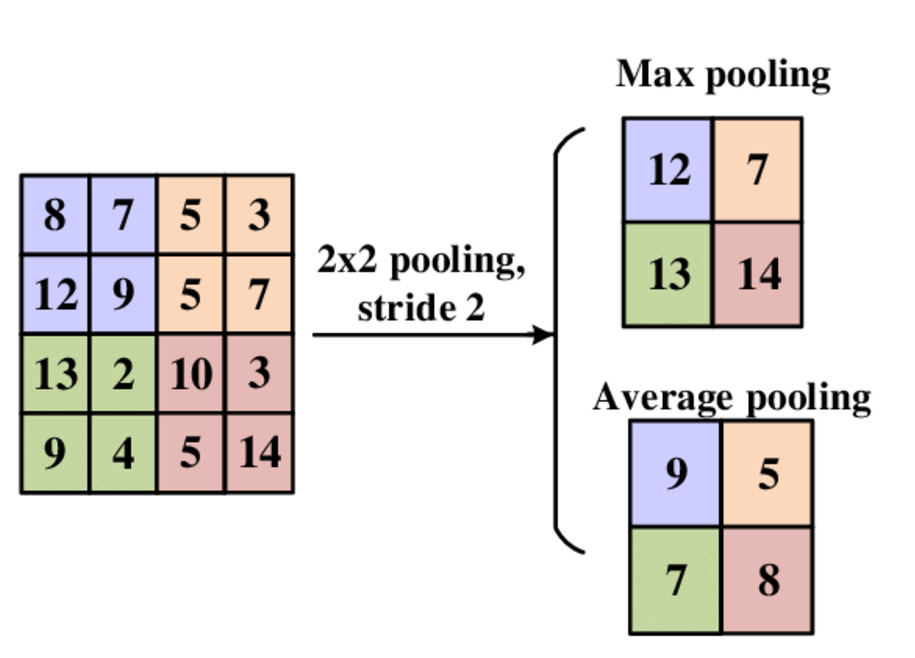
\includegraphics[scale = 0.4]{Cap2/poolinglayer.eps}
	\caption{Example of max and average pooling. Source: \citen{poolinglayer}.}\label{pooling1}
\end{figure}

\section{Gradient Descent}
The extremum of a multi-dimensional function $f(x)$, either maximum or minimum, will have a gradient equivalent to zero, so
\begin{equation}
	\nabla f(x) = 0.
\end{equation}

When working with high dimensional systems, the presence of saddles requires testing if the extremum point is a maximum or minimum. The idea of gradient descent is to iterate over the information obtained by differentiating $f(x)$ until it gets to a local minimum. To simplify the illustration,
\begin{equation}
	f(x) = x^2.
\end{equation}
Thus, the gradient can be defined as
\begin{equation}
	\nabla f(x) = \frac{\partial f(x)}{\partial x} \hat{\mathbf{x}},
\end{equation}
where $\mathbf{\hat{x}}$ is a unit vector. In order to find the local minimum, the idea is to follow the direction given by $-\nabla f(x)$. So, the algorithm can be generalized as
\begin{equation}
	\mathbf{x}_{k+1}(\delta) = \mathbf{x}_{k} - \delta \nabla f(x_{k}),
\end{equation}	
where $\delta$ is the parameter that dictates how far each ``step'' goes. Figure \ref{GDesc} illustrates the Gradient descent finding a local minimum for different values of $\delta$.
\begin{figure}[h]
	\centering
	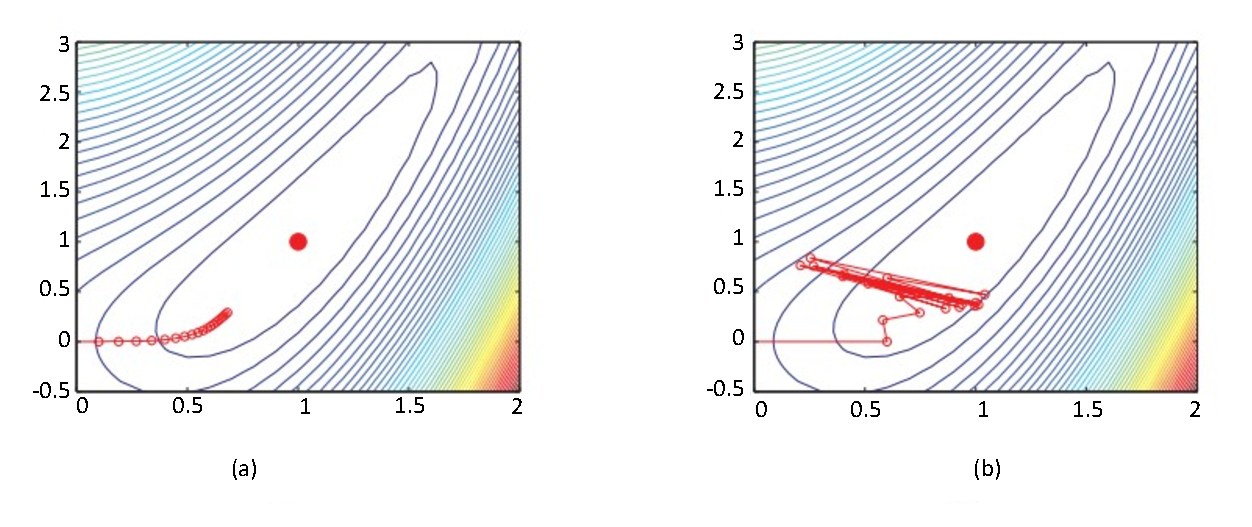
\includegraphics[scale = 0.6]{Cap2/GD.eps}
	\caption{Gradient descent on a simple function for different $\delta$. Source: \citen{Murphy-2012}.}\label{GDesc}
\end{figure}

\section{Backpropagation Algorithm}
\label{Backpropagation Algorithm}
The backpropagation algorithm (backprop) exploits the compositional nature of NNs in order to frame an optimization problem for determining the weights of the network \cite{Brunton_Kutz_2022}. In simple words, backprop is a efficient gradient estimation method that can serve as input for gradient descent. As an example, consider a NN which has one node per layer, and only one hidden layer, as shown in Figure \ref{NN_one}.

\begin{figure}[h]
	\centering
	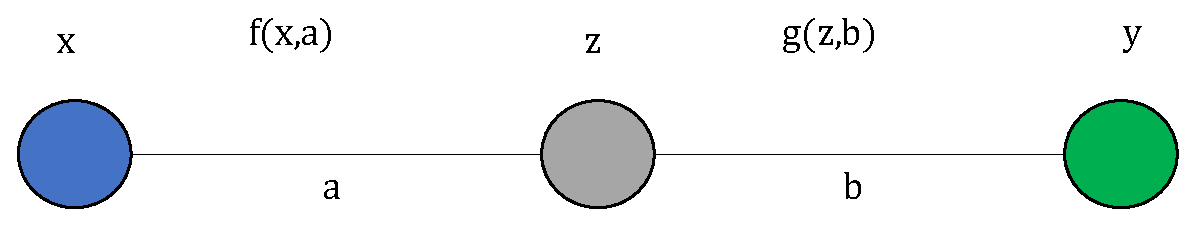
\includegraphics[scale = 0.6]{Cap2/onelayerNN.eps}
	\caption{One node per layer, one hidden layer NN. Source: \citen{Brunton_Kutz_2022}}\label{NN_one}
\end{figure}

The relation between the input and output in this NN can be described as
\begin{equation}
	y = g(z,b) = g(f(x,a),b),
\end{equation}
where $f$ and $g$ are activation functions and $a$ and $b$ the weights. Thus, the output error $E$ can be computed as
\begin{equation}
	E = \frac{1}{2}(y_{0}-y)^2,
\end{equation}
where $y_{0}$ is the correct output (imagine a labeled dataset) and $y$ is the output given by the NN. Backprop works on finding $a$ and $b$ that minimizes $E$. In this simple case, the weights are updated iterativelly
\begin{equation}
	\label{eq1}
	a_{k+1} = a_{k} - \delta \frac{\partial E}{\partial a_{k}},
\end{equation} 
\begin{equation}
	\label{eq2}
	b_{k+1} = b_{k} - \delta \frac{\partial E}{\partial b_{k}},
\end{equation}
where $\delta$ is a hyperparameter called learning rate. A full generalization of backprop can be writen as
\begin{equation}
	w^j_{k+1} = w^j_{k} - \delta \frac{\partial E}{\partial w^j_{k}},
\end{equation}
where $w^j_{k}$ can be understood as the $j$-th component of a vector $\mathbf{w}$ that contains all the elements of the matrices $\mathbf{A}_{j}$ (shown in Section \ref{Neural Networks}).

\section{Stochastic Gradient Descent Algorithm}
\label{SecaoStocastica}
As described by \citen{Brunton_Kutz_2022}, the Stochastic Gradient Descent Algorithm (SGD) has an advantage when it comes to training a NN: faster evaluation of the optimal weights. SGD estimates the gradient using a batch of a fixed number of training examples, which is less than the actual dataset (mini-batch) at each iteration. Thus, the SGD algorithm can be writen as
\begin{equation}
	\mathbf{w}_{j+1}(\delta) = \mathbf{w}_j - \delta \nabla E_k(\mathbf{w}_j),
\end{equation}
where $\mathbf{w}_{j}$ is the vector of all the network weights at the $j$-th iteration, and $k \in \left[k_1,k_2,...,k_p\right]$ denotes the $p$ selected data points $k_j$ used to approximate the gradient.

\section{Object Detection}
\citen{lin2015microsoftcococommonobjects} defines image classification as a task that requires binary labels, in order to indicate if objects are present in an image. Detecting an object involves two key tasks: confirming the presence of an object from a specified class and identifying its location within the image. The location is usually represented by a bounding box, as shown in Figure \ref{objectdetection}.

\begin{figure}[h]
	\centering
	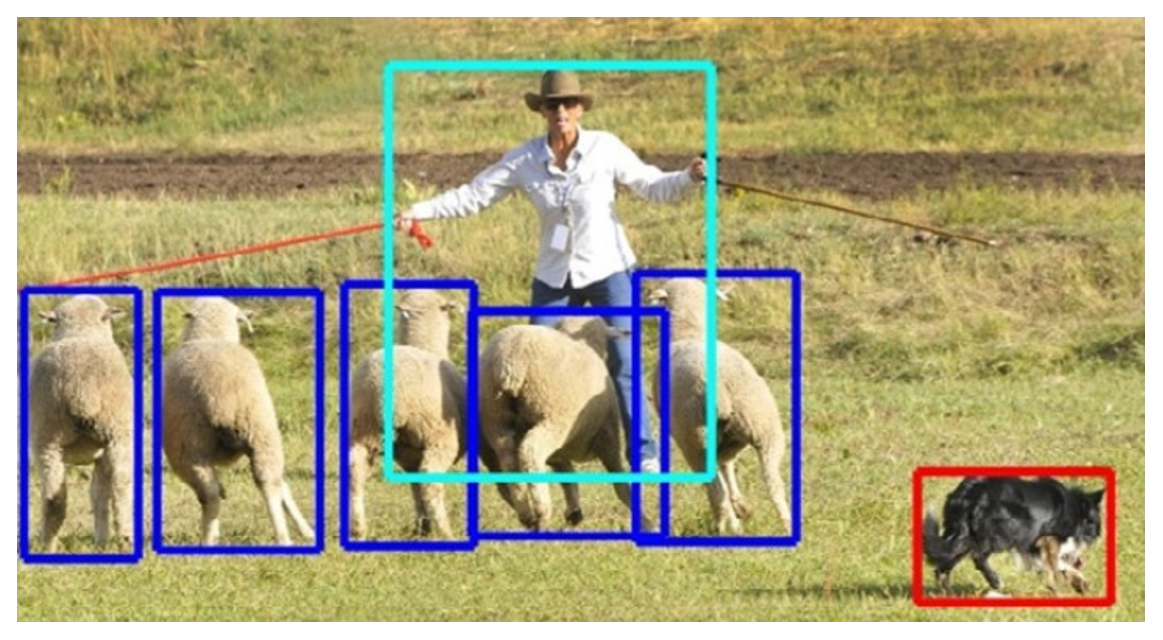
\includegraphics[scale = 0.5]{Cap2/Obj_Detec.eps}
	\caption{Object localization using bounding box. Extracted from \citen{lin2015microsoftcococommonobjects}.}\label{objectdetection}
\end{figure}

\subsection{IoU}
Intersection over Union (IoU) measures the closeness of the predicted and ground truth BBs. As the name sugests, it is the area of intersection between the predicted BB and the ground truth BB divided by the area of their union. This parameter dictates how close the predicted BB is from the ground truth and can be writen as
\begin{equation}
	IoU = \frac{\textrm{area}(B_p \cap B_{gt})}{\textrm{area}(B_p \cup B_{gt})}
\end{equation}
where $B_p$ and $B_{gt}$ are the predicted and ground truth bounding boxes, respectively. A prediction is considered correct if the predicted and ground truth BBs belongs to the same class and the IoU between them is higher than a threshold value. Predictions can be separated into four categories, as shown in Table \ref{Predictionstable}.

\begin{table}[h]
\begin{center}
\caption{Types of bounding box prediction.}
\label{Predictionstable}
\begin{tabular}{|c|m{9cm}|c|} 
 \hline
 Prediction & Description \\ [0.5ex] 
 \hline\hline
 True Positive (TP) & Model predicts a bounding box on a location and it is correct \\ 
 \hline
 False Positive (FP) & Model predicts a bounding box on a location and it is wrong \\
 \hline
 True Negative (TN) & Model does not predict a bounding box on a location and it is correct \\
 \hline
 False Negative (FN) & Model does not predict a bounding box on a location and it is wrong \\
 \hline
\end{tabular}
\end{center}
\end{table}

\subsection{Mean Average Precision}
To understand the concept of mean Average Precision (mAP), precision and recall must be defined. According to \citen{PascalVOC}, recall is defined as the proportion of all positive examples with confidence above a given threshold. Precision is the proportion of all examples above that threshold which are from the positive class. In mathematical terms,
\begin{equation}
	P = \frac{TP}{TP+FP},
\end{equation}
\begin{equation}
	R = \frac{TP}{TP+FN},
\end{equation}
where $P$ and $R$ are precision and recall, respectively. In multiclass classification, the model outputs the conditional probability that a specific bounding box belongs to one possible class. Greater probability means higher chances for the bounding box to contain that class. The probability distribution along with a user-defined confidence threshold (between 0 and 1) value is used to classify a bounding box \cite{grandini2020metricsmulticlassclassificationoverview}. A precision-recall curve plots the value of precision against recall for different confidence threshold values. To compute the Average Precision for each class, the methodology used in Pascal VOC2008 \cite{PascalVOC} divided the recall axis into eleven points $r \in [0,0.1,...,1]$ and interpolated the curve using 
\begin{equation}
	p_{\textrm{interp}}(r) = \underset{\tilde{r}:\tilde{r} \geq r}{\max p(\tilde{r})},
\end{equation}
which means to take the precision at each recall level $r$ and replace by the maximum precision measured in $\tilde{r} > r$. Figure \ref{PrecisionxRecallnet} presents an example of this interpolation on a Precision-Recall curve.

\begin{figure}[h]
	\centering
	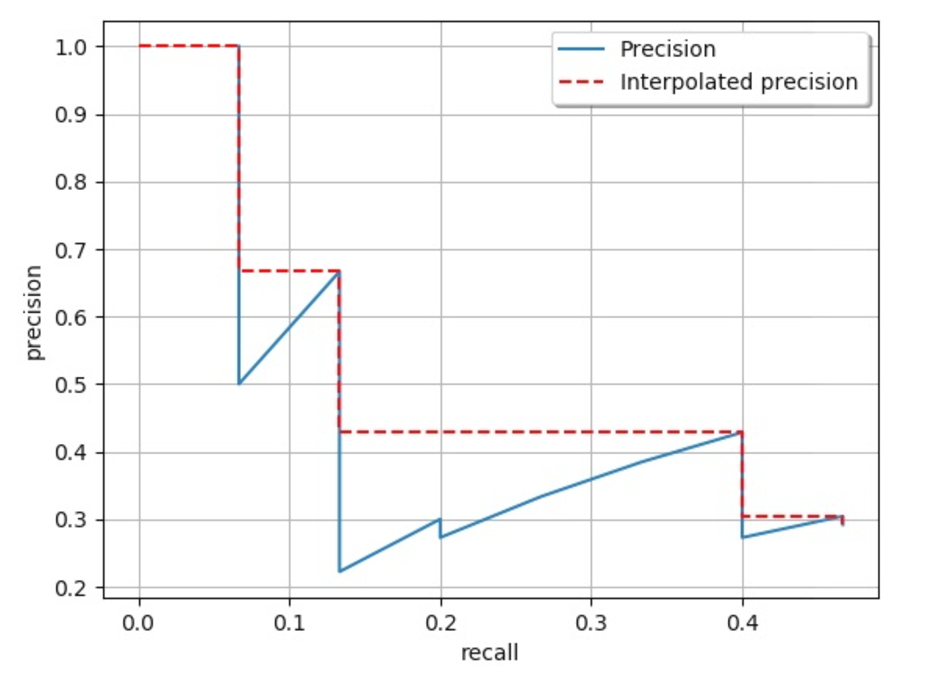
\includegraphics[scale = 0.6]{Cap2/PrecisionxRecallCurve.eps}
	\caption{Precision-Recall curve interpolation. Extracted from \citen{9145130}.}\label{PrecisionxRecallnet}
\end{figure}

The average precision $AP$ was then computed by taking the arithmetic mean of the eleven precision values $p_{\textrm{interp}}(r)$: 
\begin{equation}
	AP = \frac{1}{11}\sum_{r \in \left\{0,0.1,...,1\right\}}^{}p_{interp}(r).
\end{equation}

The mean Average Precision at a given IoU threshold t (mAP@t) can be obtained using
\begin{equation}
	mAP = \frac{1}{N}\sum_{i=1}^{N}AP_i,
\end{equation}
where $AP_i$ is the Average Precision for class $i$. The threshold $t$ can also be a range of numbers ($t = [50, 55, 60, ..., 95]$). In this case, mAP@50-95 is the mean of mAPs computed for each value in $t$.

\section{YOLO - You Only Look Once}
YOLO is a computer vision model for object detection, classification and segmentation tasks in real time. The first version was presented by \citen{YOLO}, and consists of a single CNN predicting multiple bounding boxes and class probabilities for those boxes simultaneously, as shown in Figure \ref{YOLOworking}. YOLO's first version consisted of 24 convolutional layers followed by 2 fully connected layers, as shown in Figure \ref{YOLOv1}.

 \begin{figure}[h]
	\centering
	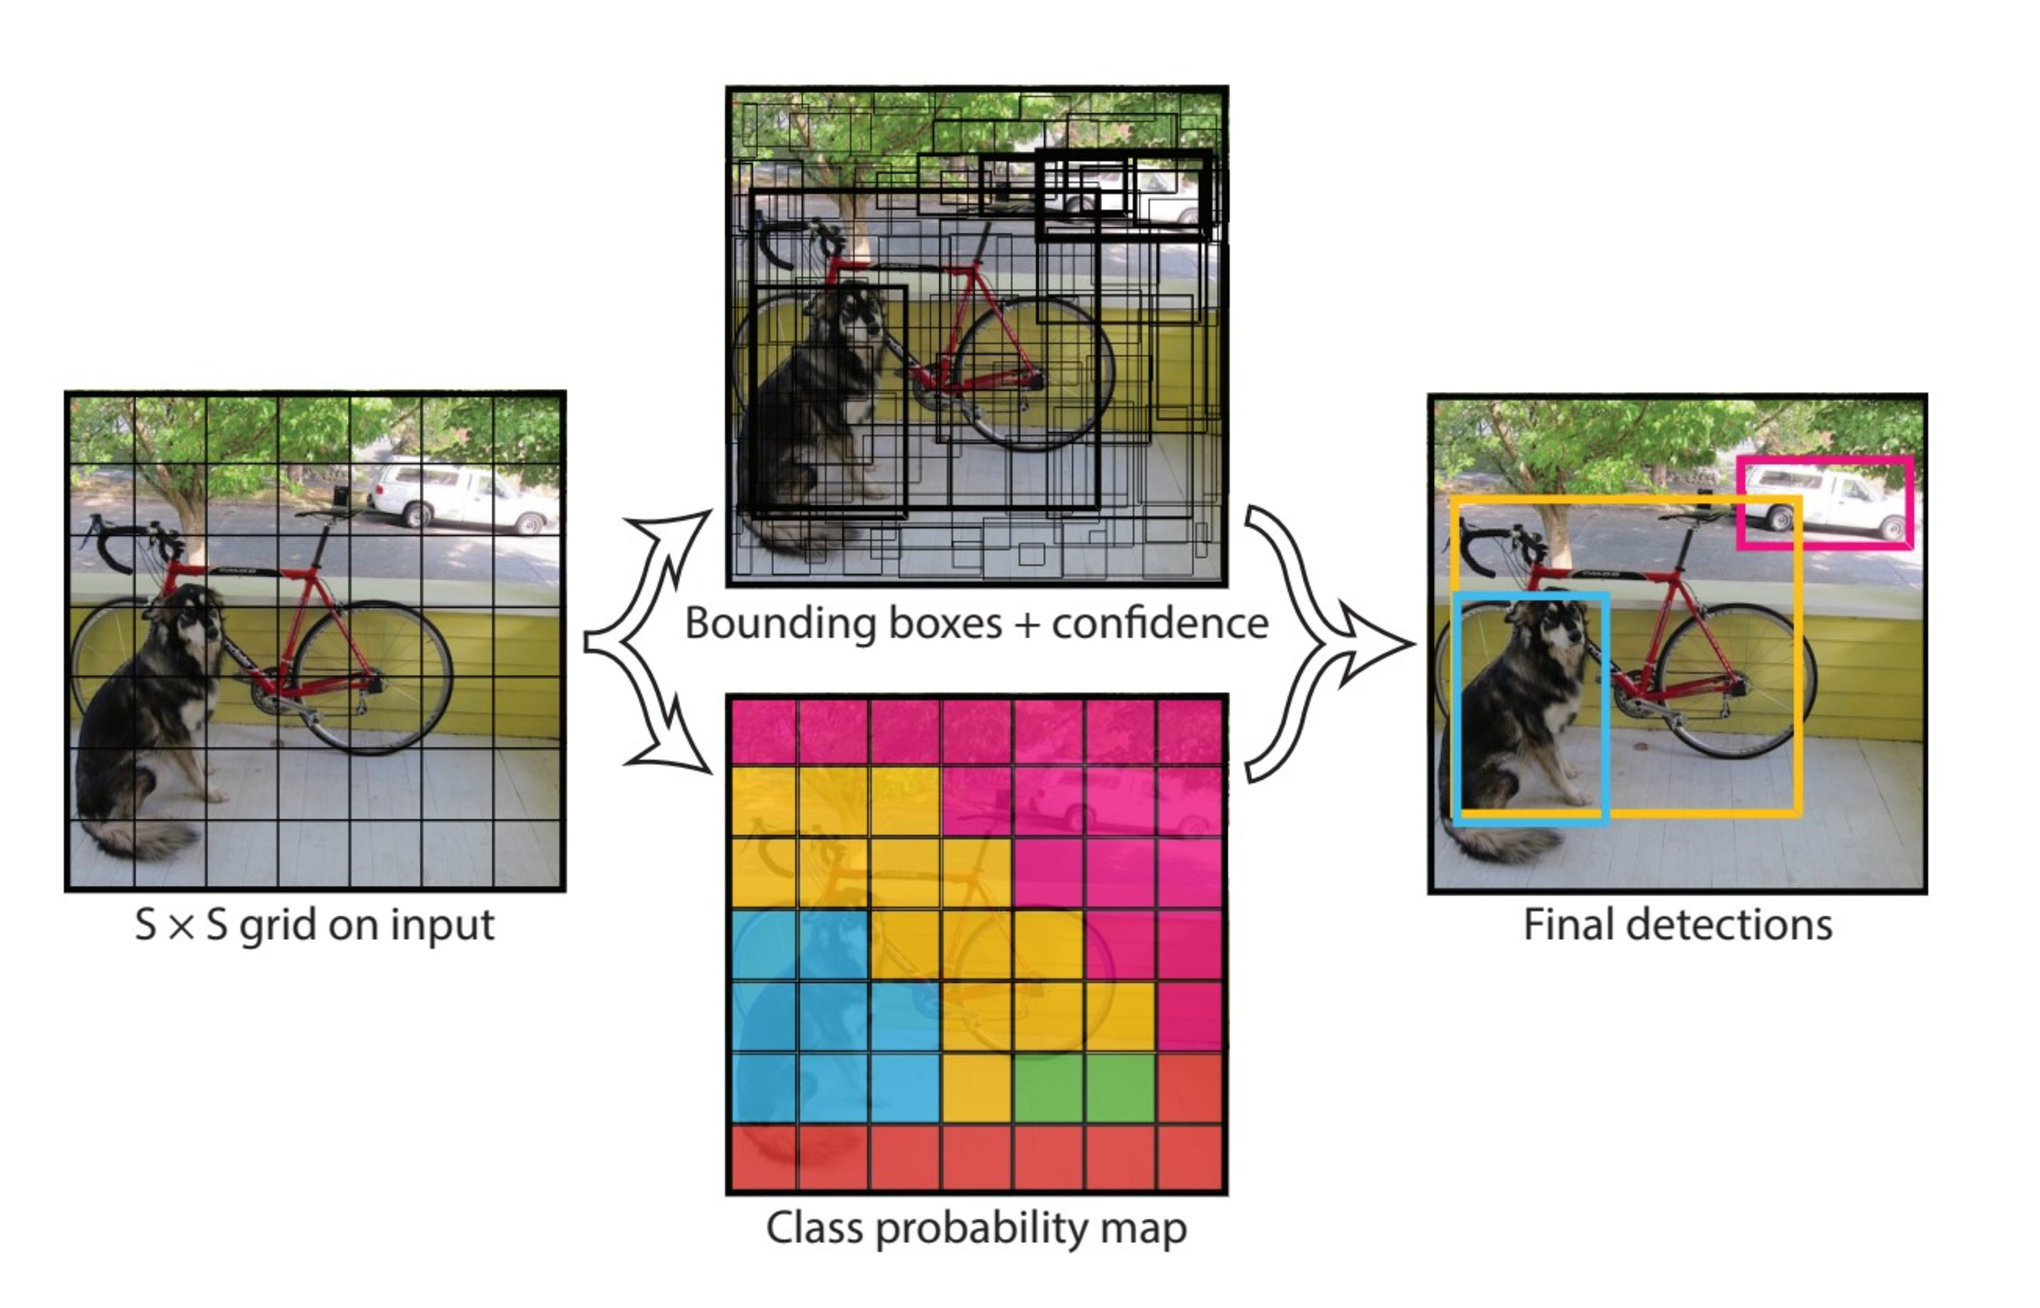
\includegraphics[scale = 0.3]{Cap2/YOLOworking.eps}
	\caption{YOLO model. Source: \citen{YOLO}.}\label{YOLOworking}
\end{figure}

 \begin{figure}[H]
 	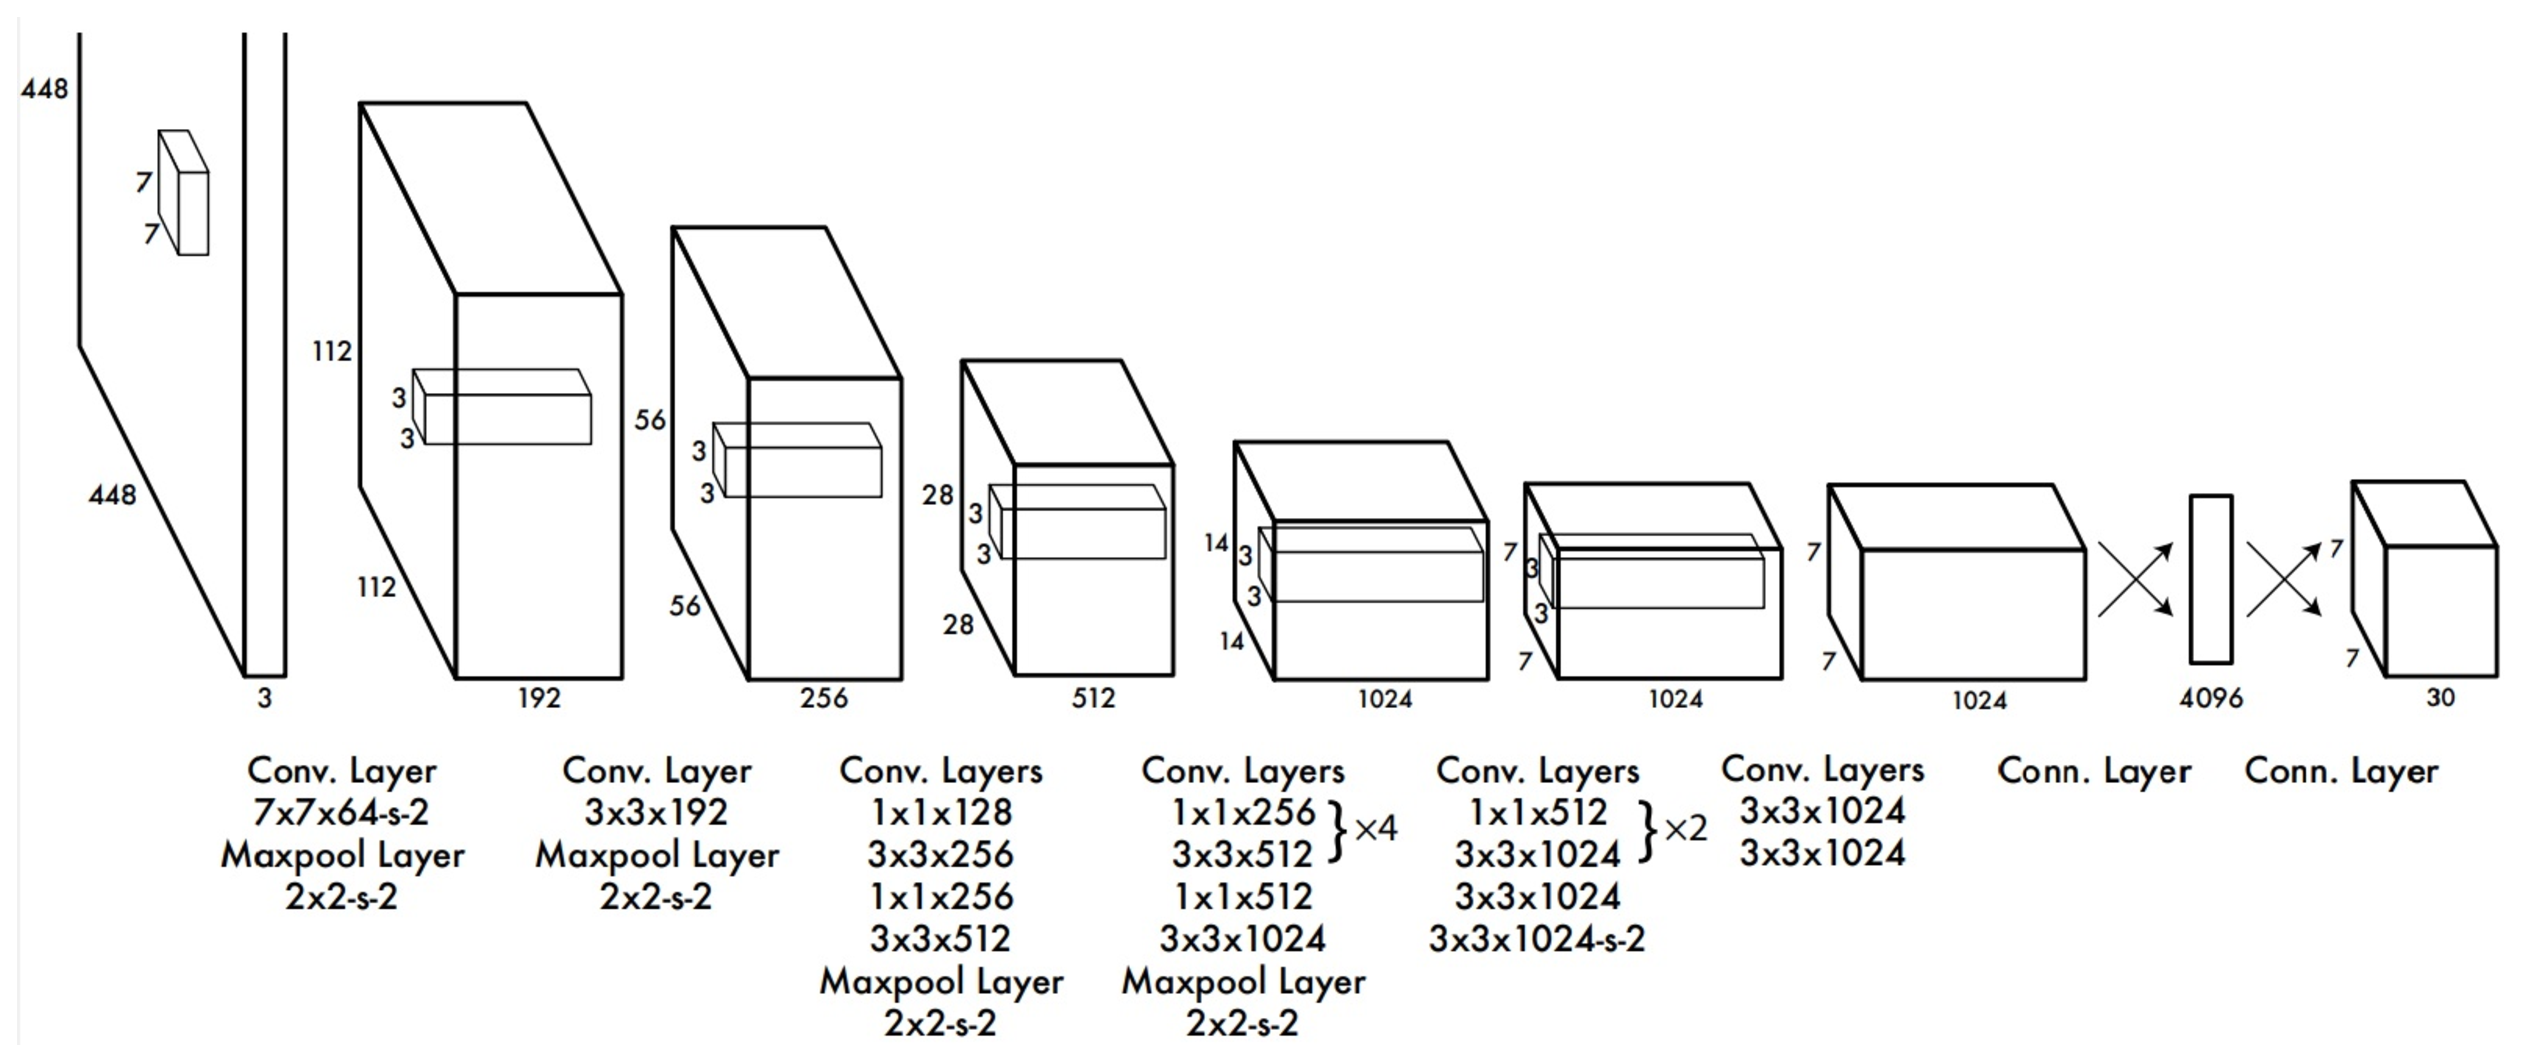
\includegraphics[scale = 0.35]{Cap2/YOLOv1.eps}
 	\caption{YOLOv1 architecture. Source: \citen{YOLO}.}\label{YOLOv1}
 \end{figure}
 
In this work we will use YOLOv8, which is described by \citen{Jocher_Ultralytics_YOLO_2023} as a model that builds upon the success of previous YOLO versions and introduces new features and improvements to further boost performance and flexibility.

\section{Kalman Filter}
\label{secaokalmanfilter}
According to Grewal and Andrews (2015), the Kalman filter is a mathematical tool used almost exclusively for two purposes: estimation and performance analysis of estimators. It works on minimizing the mean squared error between the actual and estimated data, providing the best estimation of the data in this sense. 

To explain the algorithm, we assume that we want to determine the value of a variable in the form:
\begin{equation}
	x_{k+1} = \mathbf{\Phi} x_k + w_k,
\end{equation}
where $x_k$ is the state vector at time $k$, $\mathbf{\Phi}$ is the state transitioning matrix from state $x_k$ to $x_{k+1}$ and $w_k$ is called white noise. The idea is to consider measurements on this variable modelled as
\begin{equation}
	z_k = \textbf{H} x_k + v_k,
\end{equation}
where $z_k$ is the measurement of $x$ at time $k$, $\textbf{H}$ is the connection between the state vector and the measurement vector, and $v_k$ is the associated measurement error. Now, if we consider the estimated variable $\hat{x}_k$ to be related with the measurement $z_k$ by
\begin{equation}
	\hat{x}_k = \hat{x}_k' + K_k (z_k - \textbf{H}\hat{x}_k'),
\end{equation}
where $\hat{x}_k'$ is the prior state of $\hat{x}_k$ and $K_k$ is the Kalman gain, the algorithm recursivelly update the variables according Figure \ref{Kalmanalgoritmo}, where $I$ is the identity matrix, $P_k$ is the error covariance matrix and $Q$ is the coavriance of $w_k$, given by
\begin{equation}
	P_k = E[(x_k-\hat{x}_k) (x_k-\hat{x}_k)^T],
\end{equation}
and
\begin{equation}
	Q = E[w_k w_k^T].
\end{equation}

\begin{figure}[h]
	\centering
	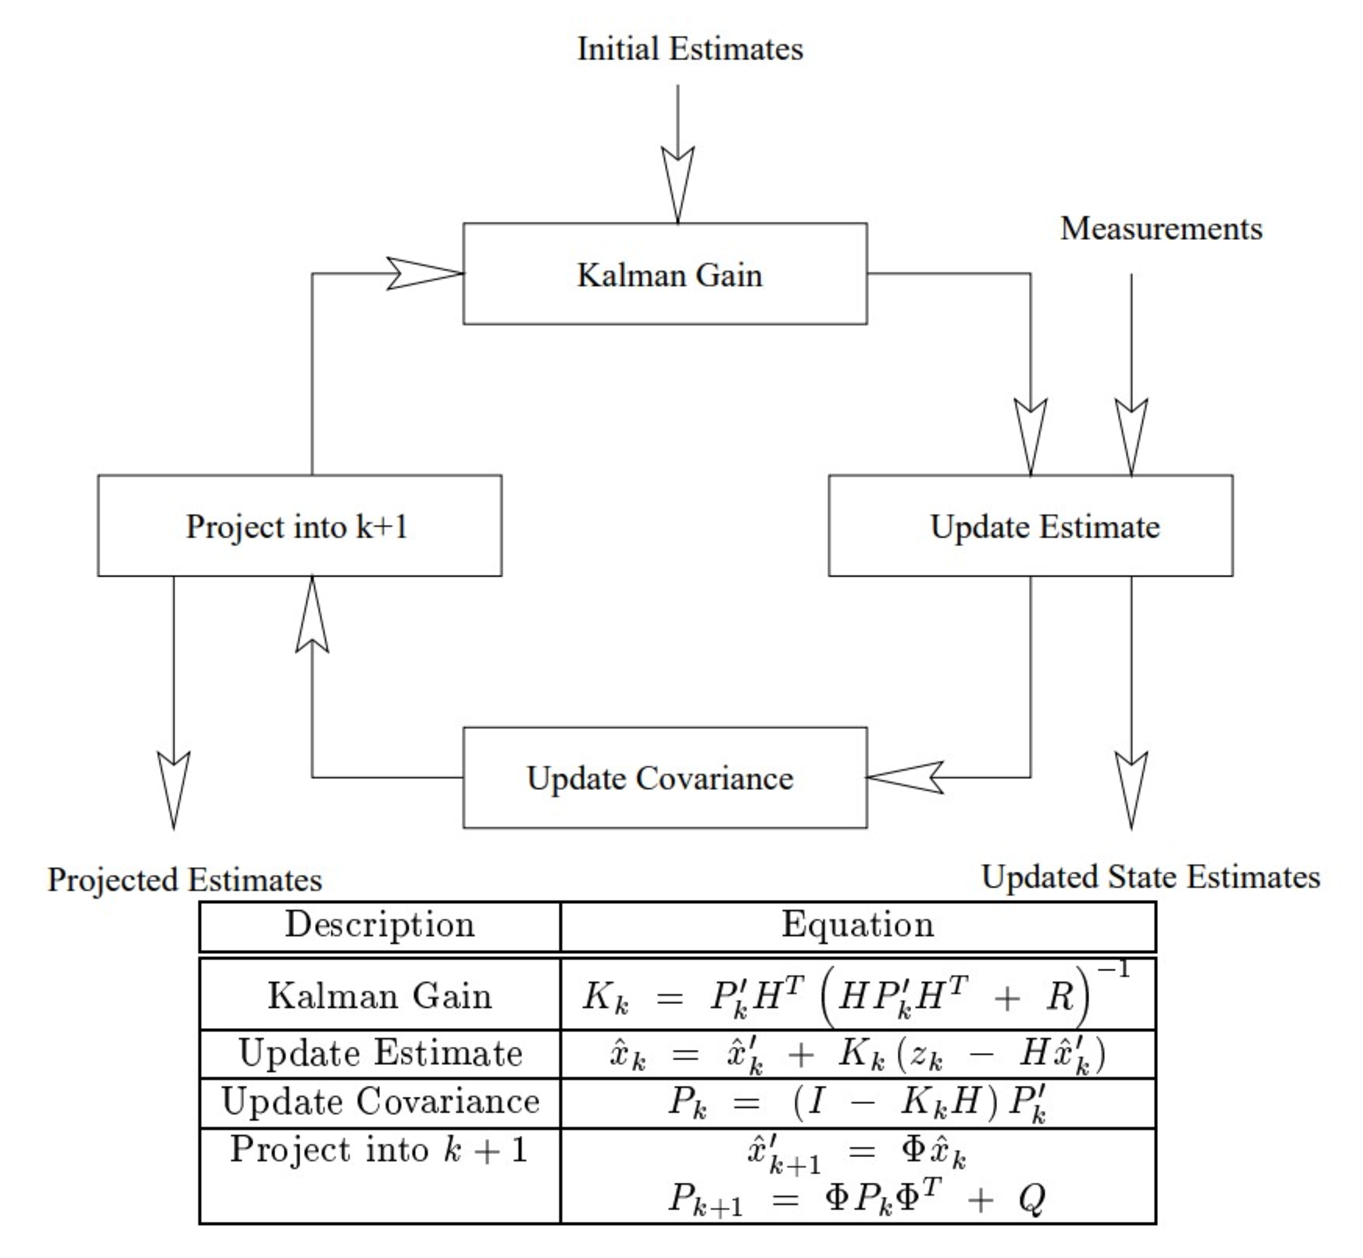
\includegraphics[scale = 0.5]{Cap2/Recursivekalman.eps}
	\caption{Kalman filter algorithm working recursivelly. Extracted from \citen{Lacey1998TutorialTK}.}\label{Kalmanalgoritmo}
\end{figure}

\section{Gimbal System}
This section describes the gimbal as a system, presenting the principles and how to mathematically model the dynamics.

\subsection{Reference Frames}
\label{secaorefframes}
To understand and accurately model a 2-DOF gimbal, it is essential to first divide the system into its primary components: the inner gimbal, the outer gimbal, and the base. The inner and outer gimbals provide movement in elevation ($\epsilon$) and azimuth ($\eta$), respectively, on their own reference frame. The base serves as the reference frame upon which the gimbals operate, and in this work, it is considered the inertial frame, meaning it is static and unaffected by external disturbances. It is assumed that all reference frames are orthogonal and their origin overlaps. Figure \ref{Gimbal2dg} illustrates the reference frames in a 2-DOF gimbal, where $\bm{u}^F_d$ represents the unit vector of reference frame ``$F$'' in direction ``$d$'', in which:
\begin{list}{}{}
	\item $\mathbf{B}$ is the reference frame fixed to the gimbal base. In our case, coincident to intertal frame (earth).
	\item $\mathbf{O}$ is the reference frame fixed to the outer gimbal.
 	\item $\mathbf{I}$ is the reference frame fixed to the inner gimbal.
 \end{list}

And the unit vectors are expressed as:
\begin{align*}
     \bm{u}_x &= \begin{bmatrix}1\\0\\0\end{bmatrix}, & \bm{u}_y &= \begin{bmatrix}0\\1\\0\end{bmatrix}, & \bm{u}_z &= \begin{bmatrix}0\\0\\1\end{bmatrix}.
\end{align*}

\begin{figure}[H]
 	\centering
 	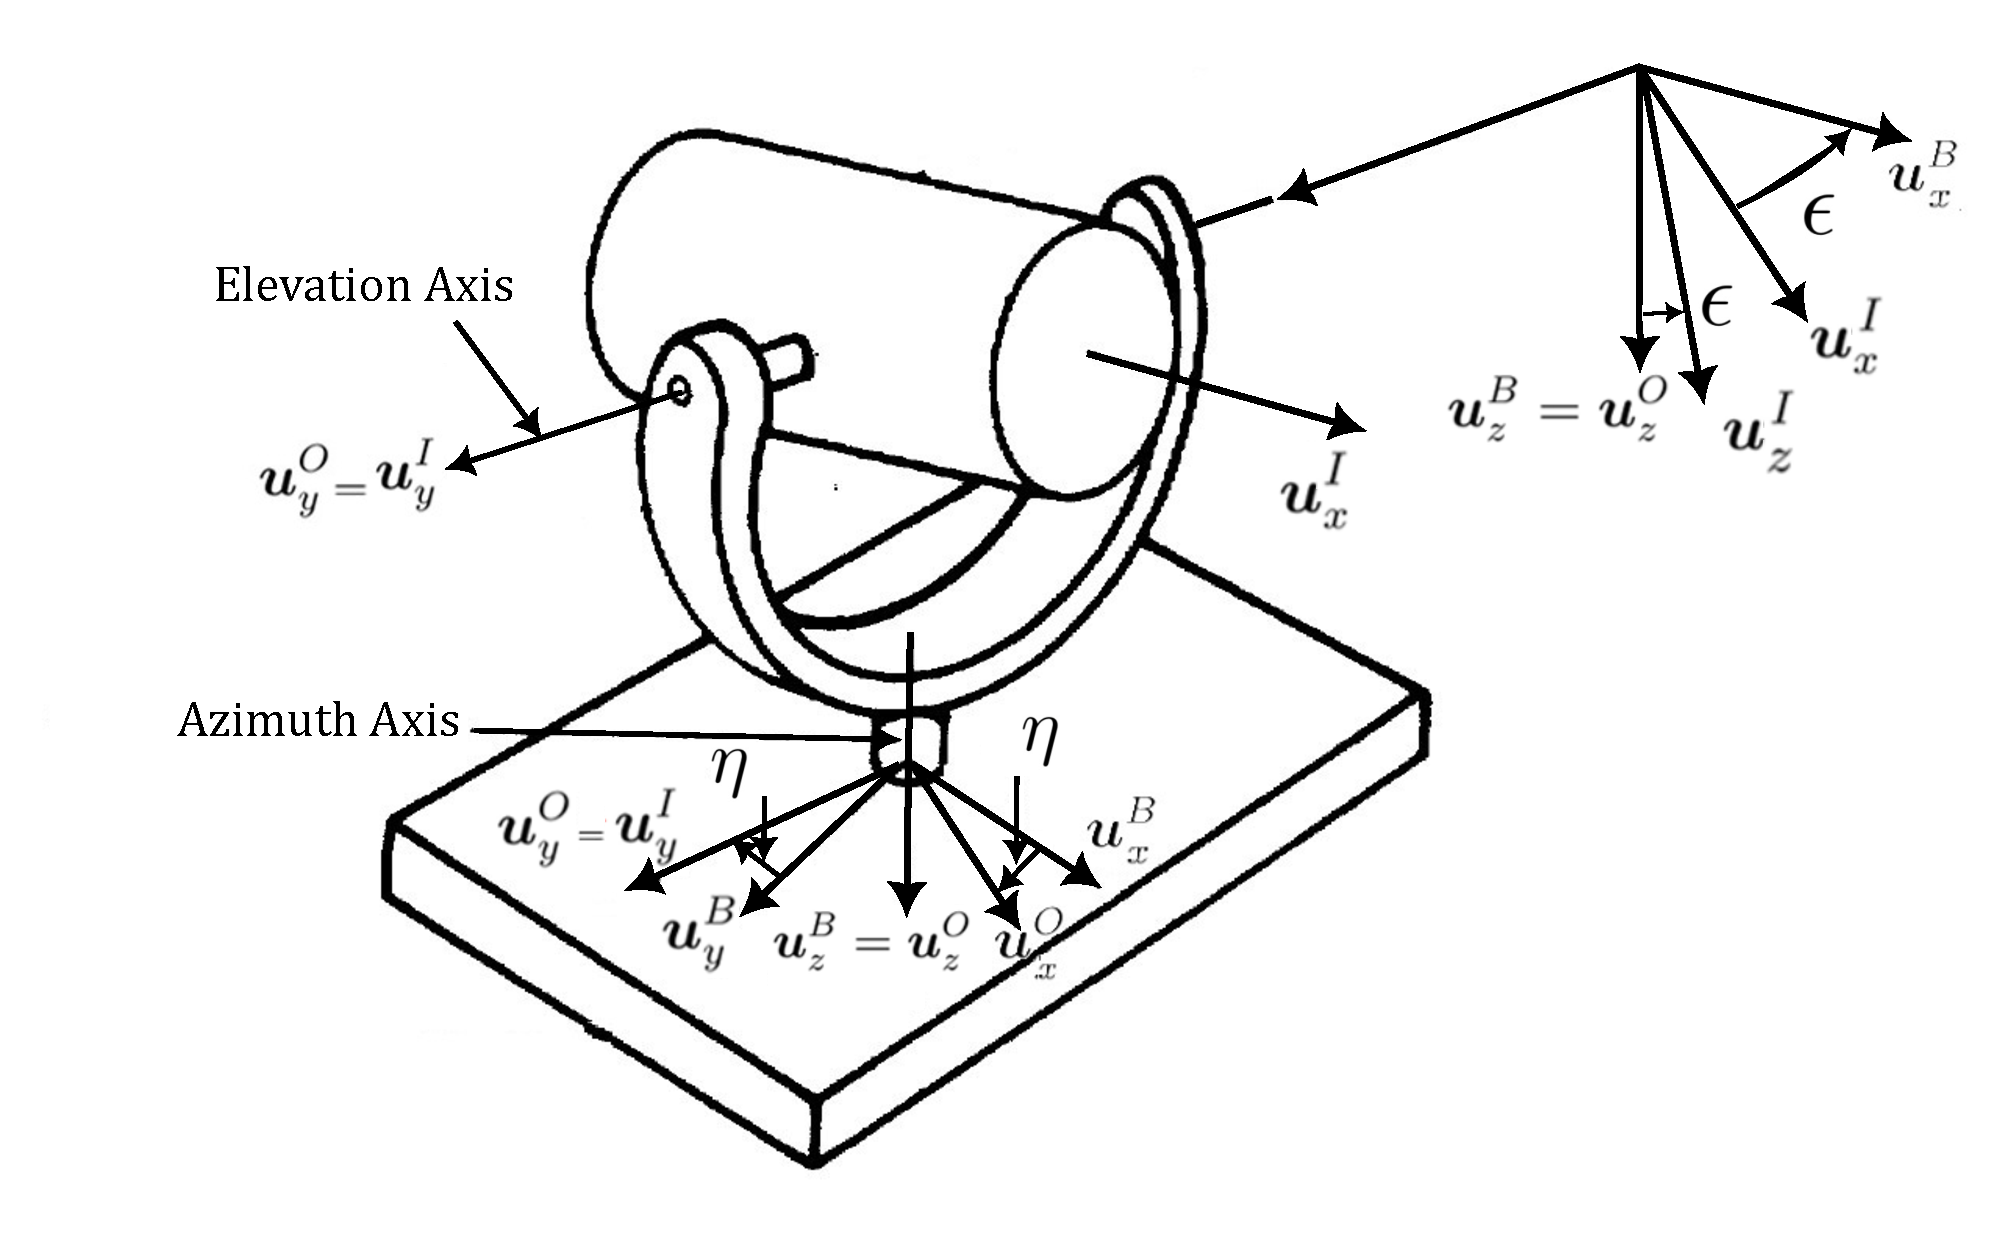
\includegraphics[scale = 0.4]{Cap6/Gimbal_final.eps}
 	\caption{Reference frames of 2-DOF Gimbal. Extracted from \citen{Gimbalmodel}}\label{Gimbal2dg}
 \end{figure}

 The relation between reference frames is estabilished by transformation matrices, which are thoroughly discussed in \citen{Done_1999}. For instance, a transformation matrix $\mathbb{T}_{F_1 F_2}$ projects a vector from reference frame $F_1$ to reference frame $F_2$. Taking into account that our system is not affected by disturbances in the base $B$, the transformation matrices applied are:

 \begin{equation}
    \mathbb{T}_{BO}(\eta) = \mathbb{T}^T_{OB}(\eta) = \left[\begin{matrix} \cos(\eta) & -\sin(\eta) & 0 \\ \sin(\eta) & \cos(\eta) & 0 \\ 0 & 0 & 1 \end{matrix}\right],
 \end{equation}

  \begin{equation}
    \mathbb{T}_{OI}(\epsilon) = \mathbb{T}^T_{IO}(\epsilon) = \left[\begin{matrix} \cos(\epsilon) & 0 & \sin(\epsilon) \\ 0 & 1 & 0 \\ -\sin(\epsilon) & 0 & \cos(\epsilon) \end{matrix}\right].
 \end{equation}

 Given the orthogonal nature of reference frames, a fundamental characteristic of transformation matrices is observed: the multiplication of a transformation matrix by its transpose invariably produces the identity matrix ($\mathbf{I}$):

\begin{equation}
   \label{equacaoidentidade}
   \mathbb{T}^T\mathbb{T} = \mathbf{I}.
\end{equation}

 \subsection{Kinematics}
 The Kinematics of the gimbal refer to the angular velocity and accelaration terms, which can be represented by 12 equations. To represent the inner and outer gimbal kinematics related to the inertial frame, the frames must be transformed to the reference frame of the gimbal base. A more detailed explanation is given in \citen{poyrazoglu_2017}.
 
 \subsubsection{Angular Velocity}
To express the velocity of each gimbal, firstly we stabilish the reference, which in our case will the the base (or inertial) frame. Hence, the velocity vector of inner and outer gimbals will be expressed as $\mathbf{\Omega}_{IB} = [\Omega_{IB_x},\Omega_{IB_y},\Omega_{IB_z}]^T$ and $\mathbf{\Omega}_{OB} = [\Omega_{OB_x},\Omega_{OB_y},\Omega_{OB_z}]^T$, respectively. Therefore, the velocity vectors can be written as

\begin{equation}
   \label{equacaoOB}
   \Omega_{OB_x} = 0,
\end{equation}

\begin{equation}
   \Omega_{OB_y} = 0,
\end{equation}

\begin{equation}
   \Omega_{OB_z} = \dot \eta,
\end{equation}

for the outer gimbal, and

\begin{equation}
   \mathbf{\Omega}_{IB} = \dot \epsilon \bm{u}_y + \mathbb{T}_{IO}(\epsilon)  \mathbf{\Omega}_{OB} = \dot \epsilon \bm{u}_y + \mathbb{T}_{IO}(\epsilon)  \dot \eta \bm{u}_z,
\end{equation}

\begin{equation}
   \Omega_{IB_x} = -\dot \eta sin(\epsilon),
\end{equation}

\begin{equation}
   \Omega_{IB_y} = \dot \epsilon,
\end{equation}

\begin{equation}
   \label{equacaoIB}
   \Omega_{IB_z} = \dot \eta cos(\epsilon),
\end{equation}

for the inner gimbal. Therefore, the resultant vectors can be expressed as

 \begin{equation}
    \mathbf{\Omega}_{OB} = \left[\begin{matrix} 0 \\ 0 \\ \dot \eta \end{matrix}\right],
 \end{equation}

 \begin{equation}
    \mathbf{\Omega}_{IB} = \left[\begin{matrix} -\dot \eta sin(\epsilon) \\ \dot \epsilon \\ \dot \eta cos(\epsilon) \end{matrix}\right].
 \end{equation}

 \subsubsection{Angular Acceleration}
The anglar acceleration is obtained by taking the first derivative of the velocity vector $\mathbf{\Omega}$ with respect to time. The angular acceleration of frame $F_1$ in relation to $F_2$ is expressed as $\bm{\alpha}_{F_1 F_2}$ = $[\alpha_{{F_1 F_2}_x}, \alpha_{{F_1 F_2}_y}, \alpha_{{F_1 F_2}_z}$]$^T$ .Therefore, the angular acceration vectors for our system are:

\begin{equation}
   \alpha_{OB_x} = 0,
\end{equation}

\begin{equation}
   \alpha_{OB_y} = 0,
\end{equation}

\begin{equation}
   \alpha_{OB_z} = \ddot \eta,
\end{equation}

and

\begin{equation}
   \alpha_{IB_x} = - (\ddot \eta sin(\epsilon) + \dot \eta \dot \epsilon cos(\epsilon)),
\end{equation}

\begin{equation}
   \alpha_{IB_y} = \ddot \epsilon,
\end{equation}

\begin{equation}
   \label{alphaelevacao}
   \alpha_{IB_z} = \ddot \eta cos(\epsilon) - \dot \eta \dot \epsilon sin(\epsilon).
\end{equation}

\subsection{Friction Model}
Friction between moving components represents a significant and often nonlinear dynamic effect within mechanical systems, particularly prevalent in gimbal platforms. Friction is inherently present in the bearings supporting both the inner and outer gimbal axes, and its influence becomes particularly pronounced during changes in the direction of rotation.

For modeling purposes, the total friction force (or torque) can be broadly categorized into two primary types: viscous friction and Coulomb friction. The overall friction torque ($T_{\text{friction}}$) acting on the system is thus expressed as the sum of these two components:

\begin{equation*}
T_{\text{friction}} = T_{\text{viscous}} + T_{\text{coulomb}},
\end{equation*}
where $T_{viscous}$ denotes the viscous friction torque and $T_{coulomb}$ represents the Coulomb friction torque. Viscous friction is characterized by its proportionality to the relative velocity between the moving surfaces, while Coulomb friction is nonlinear in nature and is primarily based on the friction between two objects resulting from the applied normal force. In \citen{espinosa2016diseno}, these friction components are mathematically formulated as:
    \begin{equation}
      \label{atritoviscoso}
    T_{\text{viscous}} = k_{\text{vf}} \Omega,
    \end{equation}
    where $k_{\text{vf}}$ is the viscous friction coefficient between the moving parts in the gimbal system, and ${\Omega}$ represents the angular velocity rotating body (inner or outer gimbal), and
    \begin{equation}
      \label{atritocoulomb}
    T_{\text{coulomb}} = k_{\text{cf}} \text{sign}(\Omega),
    \end{equation}
    where $k_{\text{cf}}$ is the Coulomb friction coefficient, and $\text{sign}(\Omega)$ is the sign function of the angular velocity, ensuring that the friction torque opposes the direction of motion.

This detailed modeling of friction results in a more realistic dynamic behavior of the gimbal system, allowing for a more accurate simulation and subsequent controller design that accounts for these inherent nonlinearities.

\subsection{Gimbal Dynamics}
\label{secaodinamicagimbal}
To obtain the equations describing the gimbal's dynamics, we will employ the Newton-Euler mechanics. This approach, based on applying Newton's laws for translation and Euler's laws for rotation to each rigid body in the system, is widely used in the modeling of mechatronic and robotic systems, as detailed in works such as \citen{boiffier1998dynamics}.

The choice of the Newton-Euler method is justified by its ability to provide a direct representation of the relationships between applied forces/torques and the resulting motion, making it particularly useful for systems with rotational joints like gimbals. To simplify the derivation of the equations and focus on the central aspects of tracking control, premises are adopted regarding mass distribution and rotation axes, such as homogeneous mass distribution, which is the assumption that mass is homogeneously distributed within the gimbals and the alignment with principal axes of inertia, ensuring that the axes of rotation coincide exactly with the principal axes of inertia of each link. These simplifications implies that products of inertia are null, resulting in diagonal inertia tensors. These simplifications neglect cross-coupling terms in the inertia matrix, which would otherwise arise from mass unbalance or misalignment of principal axes, thereby simplifying the dynamic equations. Such an approach is common in initial models to reduce complexity and is explored in works such as \citen{poyrazoglu_2017} and \citen{espinosa2016diseno}, which also use this premise to simplify the modeling of gimbal dynamics. Another assumption is the fixed base, in which the base is considered fixed and represents the system's inertial reference frame. This means that no movements or external disturbances act upon the base, simplifying the kinematic and dynamic equations by eliminating terms related to the supporting platform's dynamics.

These premises allow for a clearer derivation of the fundamental equations, which will serve as the basis for the subsequent incorporation of specific nonlinearities of the system and the actuator, in line with the objective of this work.

\subsubsection{Inner Gimbal}
The angular momentum of the inner gimbal about the pivot point P relative to the inner gimbal frame is
\begin{equation}
   \mathbf{H}^I_{I,P} = \mathbb{I}^I_P \mathbf{\Omega}_{IB}.
\end{equation}

Here, $\mathbb{I}^I_P$ represents the inertia tensor of the decoupled inner gimbal, calculated about the pivot point, and $\mathbf{\Omega}_{IB}$ denotes the inner gimbal's angular velocity vector relative to the Earth frame. The total moment exerted on the inner gimbal is obtained from the first-order time derivative of its angular momentum. Building upon calculations presented in \citen{boiffier1998dynamics}, Euler's equation for the inner gimbal, specifically about its pivot point, is thus formulated as:
\begin{equation}
   \label{momento total}
   \mathbf{M}_{OI} = \frac{d\mathbf{H}^O_{I,P}}{dt} = \mathbb{I}^I_P \bm{\alpha}_{IB} + \mathbf{\Omega}_{IB} \times \mathbf{H}^I_{IP}.
\end{equation}
In equation \eqref{momento total}, $\mathbf{H}^O_{I,P}$ is the angular momentum of the inner gimbal about the pivot point $P$ relative to the outer gimbal frame, and $\bm{\alpha}_{IB}$ is the inner gimbal's angular acceleration vector. Using the premises stated in the beginning of this section, the inertia tensor and, therefore, the vector representing the total moment exerted on the inner gimbal can be expressed as
\begin{equation}
   \mathbb{I}^I_P = \left[ \begin{matrix}I^I_x & 0 & 0 \\ 0 & I^I_y & 0 \\ 0 & 0 & I^I_z\end{matrix}\right],
\end{equation}
\begin{equation}
   \mathbf{M}_{OI} = \left[ \begin{matrix}I^I_x \alpha_{IB_x} + (I^I_z - I^I_y) \Omega_{IB_y} \Omega_{IB_z} \\ I^I_y \alpha_{IB_y} + (I^I_x - I^I_z) \Omega_{IB_x} \Omega_{IB_z} \\ I^I_z \alpha_{IB_z} + (I^I_y - I^I_x) \Omega_{IB_x} \Omega_{IB_y}\end{matrix}\right].
\end{equation}

Including the effects of friction torque in the total moment, and considering that torque is transfered from outer gimbal to the inner gimbal along the $y$ axis, therefore neglecting the components in $x$ and $z$ axes, the resultant vector is now
\begin{equation}
   \left[\begin{matrix} 0 \\ T_{m_I} - T_{\text{Friction}_{OI}} \\ 0\end{matrix}\right] = \left[ \begin{matrix} 0 \\ I^I_y \alpha_{IB_y} + (I^I_x - I^I_z) \Omega_{IB_x} \Omega_{IB_z} \\ 0 \end{matrix}\right],
\end{equation}
which gives us the equation for elevation torque for the angular momentum in the $y$ axis for the inner gimbal:
\begin{equation}
   \label{Momento angular y inner}
   T_{m_I} - T_{\text{Friction}_{OI}} = I^I_y \alpha_{IB_y} + (I^I_x - I^I_z) \Omega_{IB_x} \Omega_{IB_z}. 
\end{equation}

In equation \eqref{Momento angular y inner}, $T_{m_I}$ is the torque transmited from the outer gimbal to the inner gimbal by an electrical motor, and $T_{\text{Friction}_{OI}}$ is the friction torque between outer and inner gimbals.

\subsubsection{Outer Gimbal}
The angular momentum of the outer gimbal about the pivot point P relative to the outer gimbal frame is

\begin{equation}
   \mathbf{H}^O_{O,P} = \mathbb{I}^O_P \mathbf{\Omega}_{OB} + \mathbb{T}_{IO} \mathbf{H}^I_{I,P}.
\end{equation}

Here, $\mathbb{I}^O_P$ represents the inertia tensor of the decoupled outer gimbal, calculated about the pivot point, and $\mathbf{\Omega}_{OB}$ denotes the outer gimbal's angular velocity vector relative to the Earth frame. Notice that this equation already consider the influence of the inner gimbal in the outer gimbal's angular moment. Applying the same considerations used in equation \eqref{momento total}, Euler's equation of the outer gimbal about the pivot point is expressed as
\begin{equation}
\mathbf{M}_{BO} + \mathbf{M}_{IO} = \frac{d\bm{H}^B_{O,P}}{dt},
\end{equation}

\begin{equation}
   \label{momento total outer gimbal}
   \frac{d\bm{H}^B_{O,P}}{dt} = \mathbb{I}^O_P \bm{\alpha}_{OB} + \mathbb{\dot T}_{IO} \mathbb{I}^I_P \bm{\Omega}_{IB} + \mathbb{T}_{IO} \mathbb{I}^I_P \bm{\alpha}_{IB} + \bm{\Omega}_{OB} \times (\mathbb{I}^O_P \bm{\Omega}_{OB} + \mathbb{T}_{IO} \mathbb{I}^I_P \bm{\Omega}_{IB}),
\end{equation}
where $\mathbf{H}^B_{O,P}$ is the angular momentum of the outer gimbal about the pivot point $P$ relative to the base frame. By expanding the terms in equation \eqref{momento total outer gimbal}, and under the assumption that torque is transfered from base to the outer gimbal along the $z$ axis, thus $M_{IO_x}$ = $M_{IO_y}$ = $M_{BO_x}$ = $M_{BO_y}$ = 0, the resultant vectors for $M_{BO}$ and $M_{IO}$ are:

\begin{align*}
     \mathbf{M}_{IO} &= \left[\begin{matrix}0 \\ 0 \\ T_{\text{Friction}_{IO}}\end{matrix}\right], & \mathbf{M}_{BO} &= \left[\begin{matrix}0 \\ 0 \\ T_{m_O} - T_{\text{Friction}_{BO}}\end{matrix}\right].
\end{align*}

In this case, $T_{\text{Friction}_{BO}}$ indicate the friction torques between the base and the outer gimbal, while $T_{m_O}$ being the motor torque applied to the outer gimbal. $T_{\text{Friction}_{IO}}$ is the influence that the friction torque between inner and outer gimbals exerts on outer gimbal's motion, and will be considered to be zero for simplification purposes. Due to the alignment of the rotation axes of the base and the outer gimbal along the $z$ axis, the sum of $T_{m_O}$ and $T_{\text{Friction}_{BO}}$ is directly transmitted to the outer gimbal, whereas $T_{\text{Friction}_{IO}}$ is a friction torque transferred indirectly. Therefore, the equation of motion for the outer gimbal on the $z$ axis is given by
\begin{equation}
\label{movimento rotacional outer gimbal}
\begin{split}
    T_{m_O} - T_{\text{Friction}_{BO}} &= I^O_z \alpha_{{OB}_z} + I^I_z \alpha_{{IB}_z} \cos(\epsilon) + I^I_x \alpha_{{IB}_x} \sin(\epsilon) \\
    &\quad - I^I_x \Omega_{{IB}_x} \Omega_{{IB}_y} \cos(\epsilon) + I^I_z\Omega_{{IB}_z} \Omega_{{IB}_y} \sin(\epsilon).
\end{split}
\end{equation}
